
%(BEGIN_QUESTION)
% Copyright 2008, Tony R. Kuphaldt, released under the Creative Commons Attribution License (v 1.0)
% This means you may do almost anything with this work of mine, so long as you give me proper credit

An analog-to-digital converter (ADC) circuit takes an analog input voltage and converts it to an equivalent digital number output.  In the following diagram, the ADC inputs an analog voltage between 0 and 5 volts DC and outputs a 10-bit binary value between {\tt 0000000000} (at exactly 0 volts input) and {\tt 1111111111} (at exactly 5 volts input).  Expressing these digital output values in decimal form, the output is 0 ``counts'' at 0 volts DC input, and 1023 ``counts'' at 5 volts DC input:

$$\includegraphics[width=15.5cm]{i03299x01.eps}$$

Determine the output of this ADC when it sees an input voltage of 2.502 volts.  Express your answer in binary, decimal, and hexadecimal forms.  Be sure to show all your work!

\vskip 30pt

Counts (binary) = 

\vskip 20pt

Counts (decimal) = 

\vskip 20pt

Counts (hexadecimal) = 

\vfil 

\underbar{file i03299}
\eject
%(END_QUESTION)





%(BEGIN_ANSWER)

This is a graded question -- no answers or hints given!

%(END_ANSWER)





%(BEGIN_NOTES)

Counts (binary) = {\tt 1000000000} or {\tt 0111111111}, depending on rounding

\vskip 10pt

Counts (decimal) = 512 or 511, depending on rounding

\vskip 10pt

Counts (hexadecimal) = \$200 or \$1FF, depending on rounding

\vskip 10pt

It is important to note that the count value output by any ADC will {\it always} be a whole number, never a fraction or a decimal.  A 10-bit converter such as this one has a count range of 0 to 1023 in whole-number steps only!

Whether or not an ADC rounds up to the next whole-number value or rounds down to the next whole-number value is impossible to determine from what little information we have here.  Some ADC designs always round down.  Some always round up.  Some alternate between the two adjacent whole-number values.  This is why either answer of the two answers shown for count value are perfectly acceptable: without knowing how the ADC is internally constructed, one cannot tell how it will round the result.

%INDEX% Mathematics review: binary-to-hexadecimal conversion

%(END_NOTES)


